\chapter{Choice of the Kinematic Reconstruction Solution with the Smallest M($t\bar{t}$)}\label{appendix:mtt}

Only the solution of the kinematic equations \ref{alg:LS1}-\ref{alg:LS6} with minimal $m(t\bar{t})$ is taken for the further analysis.
The studies which show the advisability of this criterion were performed.

The studies were performed on the generated events. The correct solution of the kinematic equations was defined by comparing the 
solution neutrino momentum $p_{\nu/\bar{\nu}}^{sol}$ to the generated one $p_{\nu/\bar{\nu}}^{gen}$ with the help of the $\chi^{2}$ criterion as following \cite{Sonnenschein:2005ed}:

\begin{equation}
 \chi^{2} = (p_{\nu_{x}}^{gen} - p_{\nu_{x}}^{sol})^{2} + (p_{\nu_{y}}^{gen} - p_{\nu_{y}}^{sol})^{2} + (p_{\nu_{z}}^{gen} - p_{\nu_{z}}^{sol})^{2} + (p_{\bar{\nu}_{x}}^{gen} - p_{\bar{\nu}_{x}}^{sol})^{2} +
 (p_{\bar{\nu}_{y}}^{gen} - p_{\bar{\nu}_{y}}^{sol})^{2} + (p_{\bar{\nu}_{z}}^{gen} - p_{\bar{\nu}_{z}}^{sol})^{2}.
\end{equation}

The fraction of correct solutions with minimal, second minimal, third minimal and fourth minimal invariant $t\bar{t}$ mass are shown in Figure \ref{fig:corrMinMtt}. In $60\%$ of 
the cases the correct solution has a minimal $m(t\bar{t})$. One might tend to average all the solutions to increase the fraction of correct solutions. However the figures \ref{} - \ref{}
show that the RMS for the average and weighted\footnote{Wight for this study is taken according to the $m(t\bar{t})$ of the solution.} average solutions are higher then the once
of the smallest $m(t\bar{t})$.

\begin{figure}[t]
  \centering
  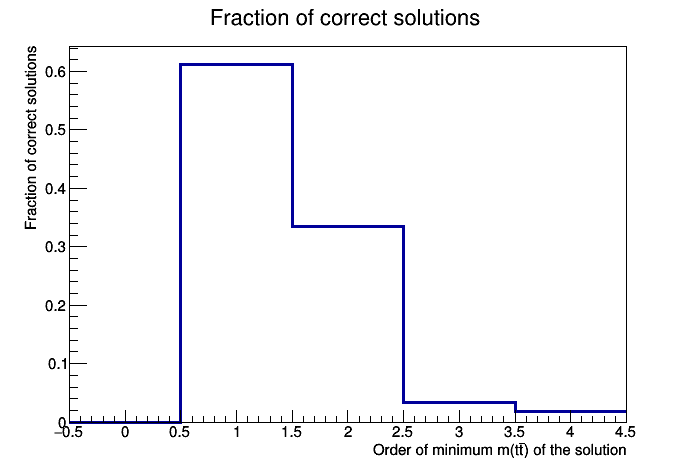
\includegraphics[width=0.8\textwidth]{10_appendices/min_Mtt/plots/corrMinMtt.png}
  \caption{Fraction of correct solutions depending on the order of minimum $m(t\bar{t})$.}
  \label{fig:corrMinMtt}
\end{figure}

